\documentclass[border=10pt]{standalone}
\usepackage{tikz}
\usetikzlibrary{positioning, shapes.geometric, calc}

\tikzset{
  box/.style={
    rectangle, rounded corners, draw=black, thick, text width=3.5cm, align=center, minimum height=0.8cm, font=\sffamily
  },
  line/.style={draw=black, thick}
}

\begin{document}
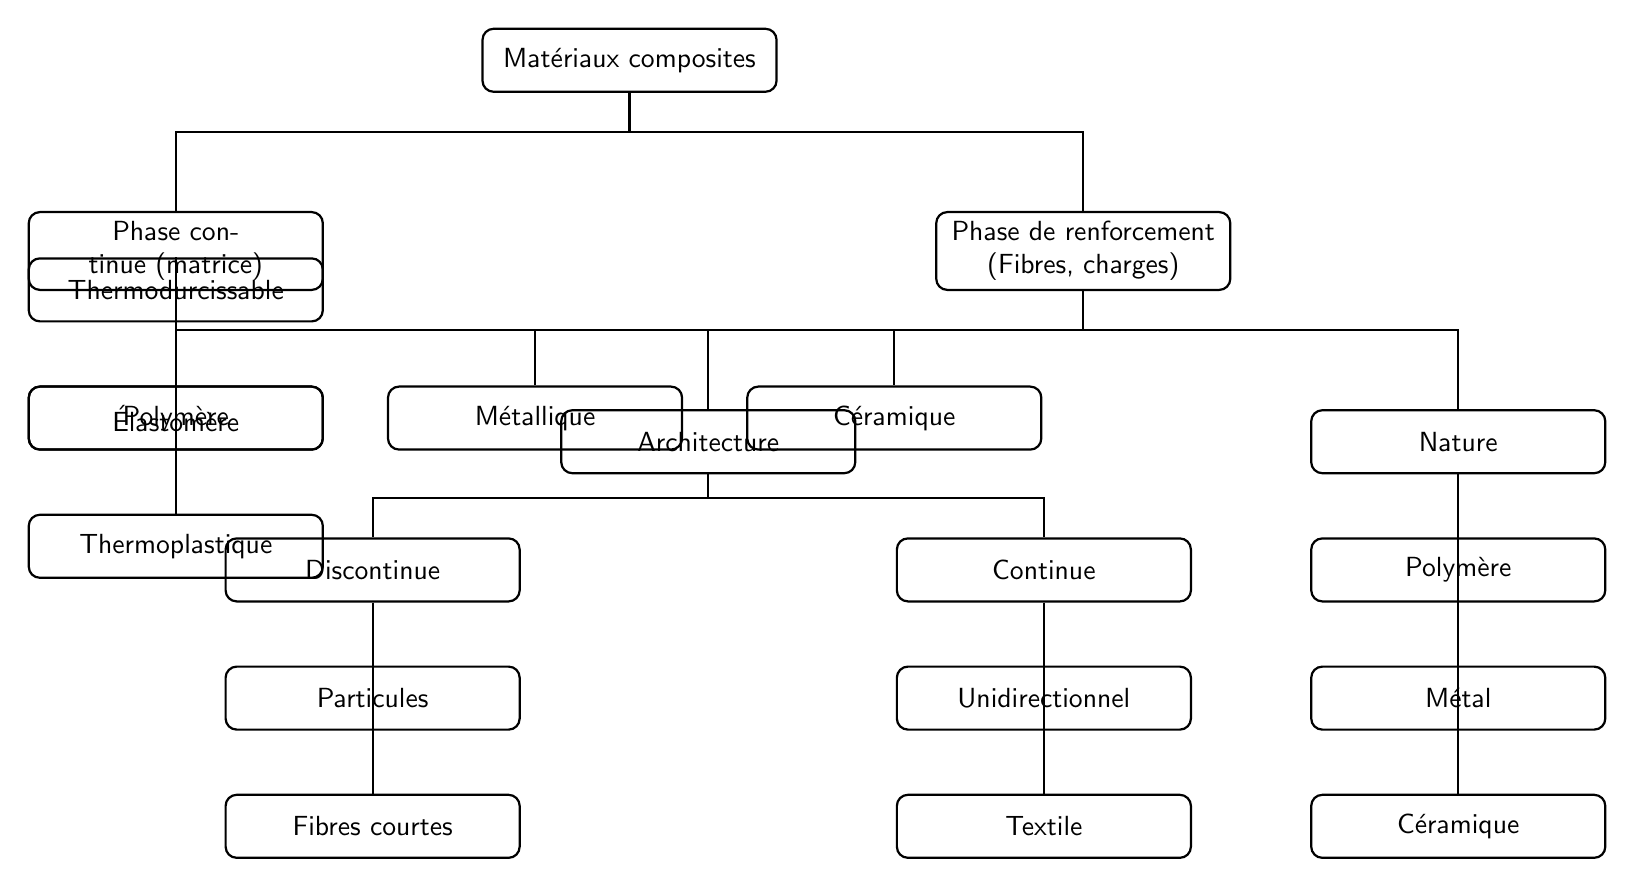
\begin{tikzpicture}[node distance=1.2cm and 0.8cm]

% Root node
\node[box] (root) {Matériaux composites};

% First level
\node[box, below left=1.5cm and 2cm of root] (phase_continue) {Phase continue (matrice)};
\node[box, below right=1.5cm and 2cm of root] (phase_renforcement) {Phase de renforcement (Fibres, charges)};

% Connect root to first level
\draw[line] (root.south) -- ++(0,-0.5) -| (phase_continue.north);
\draw[line] (root.south) -- ++(0,-0.5) -| (phase_renforcement.north);

% Phase continue branch
\node[box, below=of phase_continue] (polymere) {Polymère};
\node[box, right=of polymere] (metal) {Métallique};
\node[box, right=of metal] (ceramique) {Céramique};

\draw[line] (phase_continue.south) -- ++(0,-0.5) -| (polymere.north);
\draw[line] (phase_continue.south) -- ++(0,-0.5) -| (metal.north);
\draw[line] (phase_continue.south) -- ++(0,-0.5) -| (ceramique.north);

% Polymere subtypes
\node[box, below=0.8cm of polymere] (thermoplastique) {Thermoplastique};
\node[box, above=0.8cm of thermoplastique] (elastomere) {Élastomère};
\node[box, above=0.8cm of elastomere] (thermodurcissable) {Thermodurcissable};

\draw[line] (polymere.south) -- ++(0,-0.3) -| (thermodurcissable.north);
\draw[line] (polymere.south) -- ++(0,-0.3) -| (elastomere.north);
\draw[line] (polymere.south) -- ++(0,-0.3) -| (thermoplastique.north);

% Phase reinforcement branch
\node[box, below left=1.5cm and 1cm of phase_renforcement] (architecture) {Architecture};
\node[box, below right=1.5cm and 1cm of phase_renforcement] (nature) {Nature};

\draw[line] (phase_renforcement.south) -- ++(0,-0.5) -| (architecture.north);
\draw[line] (phase_renforcement.south) -- ++(0,-0.5) -| (nature.north);

% Architecture subtypes
\node[box, below left=0.8cm and 0.5cm of architecture] (discontinue) {Discontinue};
\node[box, below right=0.8cm and 0.5cm of architecture] (continue) {Continue};

\draw[line] (architecture.south) -- ++(0,-0.3) -| (discontinue.north);
\draw[line] (architecture.south) -- ++(0,-0.3) -| (continue.north);

% Discontinue subtypes
\node[box, below=0.8cm of discontinue] (particules) {Particules};
\node[box, below=0.8cm of particules] (fibres_courtes) {Fibres courtes};

\draw[line] (discontinue.south) -- ++(0,-0.3) -| (particules.north);
\draw[line] (discontinue.south) -- ++(0,-0.3) -| (fibres_courtes.north);

% Continue subtypes
\node[box, below=0.8cm of continue] (unidirectionnel) {Unidirectionnel};
\node[box, below=0.8cm of unidirectionnel] (textile) {Textile};

\draw[line] (continue.south) -- ++(0,-0.3) -| (unidirectionnel.north);
\draw[line] (continue.south) -- ++(0,-0.3) -| (textile.north);

% Nature subtypes
\node[box, below=0.8cm of nature] (polymere_nature) {Polymère};
\node[box, below=0.8cm of polymere_nature] (metal_nature) {Métal};
\node[box, below=0.8cm of metal_nature] (ceramique_nature) {Céramique};

\draw[line] (nature.south) -- ++(0,-0.3) -| (polymere_nature.north);
\draw[line] (nature.south) -- ++(0,-0.3) -| (metal_nature.north);
\draw[line] (nature.south) -- ++(0,-0.3) -| (ceramique_nature.north);

\end{tikzpicture}
\end{document}